
\section{Results}\label{sec:results}

\input{figs/table:results}

\begin{figure}[!t]
    \centerline{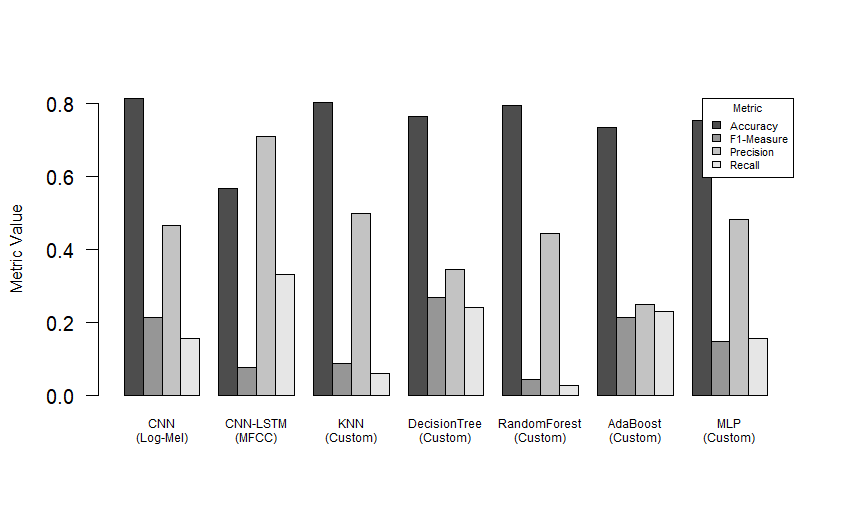
\includegraphics[width=\columnwidth]{images/perf-classifier.png}}
    \caption{Performance of Classifiers (by classification method)}
    \label{fig:perf:classifier}
\end{figure}

\begin{figure}[!t]
    \centerline{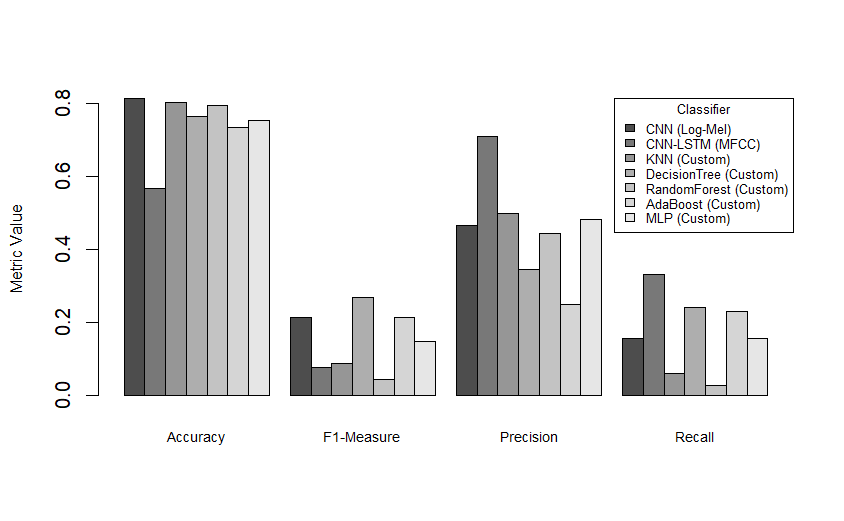
\includegraphics[width=\columnwidth]{images/perf-metric.png}}
    \caption{Performance of Classifiers (by evaluation metric)}
    \label{fig:perf:metric}
\end{figure}

Now that we have different classification results obtained from CNN, CNN-LSTM, and traditional classifiers along with different choices of feature selection, we can proceed with comparing the capability of these models to detect depression against the GRU model reported by EATD-Corpus for acoustic features.

We attempted to replicate the evaluation findings of the EATD-Corpus using an identical experimental configuration. In their original study, they reported achieving an F1-Measure of \texttt{0.66}, precision of \texttt{0.57}, and recall of \texttt{0.78}. However, our replicated results yielded an F1-Measure of \texttt{0.5112}, precision of \texttt{0.5255}, and recall of \texttt{0.5137}, indicating discrepancies compared to the reported values in the paper. This sudden drop in the reproduced results suggests that the performance of their algorithm is dependent on the random split of the folds across the K-fold cross-validation.

To ensure methodological consistency, we employed a 3-fold cross-validation approach similar to theirs for evaluating the dataset. Subsequently, we aggregated the metrics across the three folds for each classifier and calculated the average. Table~\ref{table:results} illustrates the varied metrics obtained for each classifier. We proceed to visualize the results for better intuition in  Fig.~\ref{fig:perf:classifier} and Fig.~\ref{fig:perf:metric}.

Analyzing the results of our experiments compared to the replicated results of EATD-Corpus, the following observations can be made:

\begin{itemize}[\IEEEsetlabelwidth{Z}]

    \item Considering the EATD-Corpus replicated results, it can be seen that the GRU model proposed by EATD-Corpus achieves more stable results on the Mel spectrogram features extracted from the audio files.
    
    \item The CNN network on the Log-Mel spectrogram features yields more trustable performance compared to the CNN-LSTM network on the MFCC features. While the precision and recall in the CNN-LSTM are shown to be higher, they are not trustworthy since their aggregated F1-Measure is noticeably lower than that of CNN.

    \item Although traditional machine learning classifiers applied to our custom-extracted statistical features in some cases may yield some encouraging results, overall, they struggle to accurately capture the characteristics required for effective depression detection in classifying individuals.

    \item Overall, the CNN network with Log-Mel features can be seen as a possible competitor of the EATD-Corpus. It should be reminded that the authors of EATD-Corpus utilize NetVLAD to perform dimensionality reduction and ensure fixed-length features, and they augment and resample the data to overcome data imbalance, which highly affects the evaluation results.
    
\end{itemize}

Since the target labels are expressed in terms of an SDS score (categorized using a threshold of 53 to differentiate between depressed and non-depressed), we also attempted to reframe the problem as a regression task and apply a threshold to the final numerical value instead. However, this approach yielded unsatisfactory results, leading us to exclude it from our report.
